\documentclass[master,english]{kuisthesis}
\usepackage{amsmath,amssymb,amsfonts,amsthm,enumerate,url}
\usepackage{multirow}
\usepackage{setspace}
\usepackage{array}
\usepackage[dvips]{graphicx}

\def\LATEX{{\rm (L\kern-.36em\raise.3ex\hbox{\sc a})\TeX}}
\def\LATex{\iLATEX\small}
\def\iLATEX#1{L\kern-.36em\raise.3ex\hbox{#1\bf A}\kern-.15em
    T\kern-.1667em\lower.7ex\hbox{E}\kern-.125emX}
\def\LATEXe{\ifx\LaTeXe\undefined \LaTeX 2e\else\LaTeXe\fi}
\def\LATExe{\ifx\LaTeXe\undefined \iLATEX\scriptsize 2e\else\LaTeXe\fi}
\let\EM\bf
\def\|{\verb|}
\def\<{\(\langle\)}
\def\>{\(\rangle\)}
\def\CS#1{{\tt\string#1}}

\jtitle{情報発信の対象限定性に基づくTwitterユーザの分類}
\etitle[Twitter User Classification Based on Specificity of their
Information Dissemination Target]
	{Twitter User Classification Based on Specificity of their
        Information Dissemination Target}
\jauthor{竹村 光}
\eauthor{Hikaru TAKEMURA}
\supervisor{Professor Keishi Tajima}
\date{February 7, 2014}
\department{Social Informatics}

\begin{document}
\maketitle
\begin{eabstract}

With the widespread of social media, such as blogs and social
 network services (SNS), today we have become able to publish
 information on the Web more easily than previously.  Especially
 recently, microblogging services, which are a kind of blogs coupled
 with some characteristics of SNS, has been growing explosively. As of
 2013 Octover, Twitter, which is one of the most popular microblogs, has
 over 218 million active users in the world, and as of June, more than
 500 million messages are posted on it per day.

Twitter has many characteristics of conventional social medias, so it is
 used for many purposes. Some publish information to the wide public,
 some publish information on some specific topics, and
 some communicate with their friends. Because of this characteristic,
 Twitter has attracted great attention as a new type of social media.

As explained above, Twitter is used for various purposes.  As a result,
 target specificity, the wideness of target scope of information
 publishing, varies greatly among users.  So, in this study, we propose a
 method to classify Twitter users based on target specificity of their
 information publishing.  In the method, we focus on the followers of
 the user, and classify him whether his followers are consistent in some
 noticeable characters or not.  If his followers are consistent in some
 noticeable characters, it suggests that his target specificity is high,
 i.e., he publishes information in which particular users are
 interested. On the other hand, if they are not consistent in any
 noticeable characters, there is a high possibility that the user is
 followed by a wide variety of users and it suggests that his target
 specificity is low, i.e., he publishes information in which the public
 is interested.

In addition, in this study, we focus on Twitter users whose target
 specificity is high, and we propose the method to determine why their
 target specificity is high.  In a large number of Twitter users, their
 target specificity is high and the causes vary from user to user.  For
 example, users publishing technical information about programming is
 supposed to publish information to unspecific users, but their
 target specificity is considered high because the topic of their
 publishing information is specified to certain users, i.e., users who
 are interested in programming. And also, users communicating with their
 friends or announcing to club members are supposed to publish
 information to the users specified extensionally. So their target
 specificity is supposed to be high, regardless of contents of their
 publishing information.  In the method, first, we roughly classify
 causes of target specificity into two categories: (1) because they
 publish information specified for certain topics, and (2) because they
 publish information to the users specified extensionally.  Then we
 construct classifiers which determine whether users  only belong to the
 category (1), only belong to the category (2), or belong to both (1)
 and (2), based on various features which correlate  with each category.

On the Web, it is hard to know what kinds of users each Web page
 targets to.  In Twitter, however, we can guess what kinds of users
 each user targets to by examining the followers of the user.  By using
 this information, we can determine whether a given user has high
 target specificity or not.

There are many existing studies on the classification of Twitter
 users. These studies, however, do not concern about target scope of
 information publishing.  But Twitter is used for various purposes, so
 the wideness of target scope of their information publishing varies
 greatly among users.  Following this observation, we propose a new
 classification scheme of Twitter users that focuses on target
 specificity of their information publishing.

The classification scheme of this study is supposed to apply to Twitter
 search.  In current Twitter search, messages in search results have
 various target scope of information publishing.  So it frequency
 happens that messages of certain target scope we need are buried in
 many other messages.  At that time, by using the classification of this
 study, we can search messages based on what kinds of users they target
 to.  So we can prevent messages we need from being buried in many other
 messages and find messages we need easily.

We implemented our methods with using real Twitter data, and our
 experimental results confirmed that our proposed method is effective.

\end{eabstract}

\begin{jabstract}
ブログやSNSというソーシャルメディアの普及に伴い,誰もが簡単にWeb上で情報
 を発信できるようになった.特に近年では,マイクロブログと呼ばれる,SNSの
 性質を併せ持ったブログサービスが,爆発的な成長を遂げている.最も普及し
 ているマイクロブログの1つであるTwitterでは,2012年12月現在,ユーザ数が2
 億人を超えており,同年6月現在,1日に4億以上もの記事が投稿されていると言
 われている.

Twitterは,従来の多くのソーシャルメディアの性質を兼ね合わせており,その
 利用目的が多岐に渡っている.社会のニュースのように,広く一般のユーザが
 興味を示すような情報を発信するユーザもいれば,あるトピックに特化した情
 報を発信するユーザや,友人とのコミュニケーションを行うユーザもいたりと,
 多様な利用目的のユーザが混在している.このような性質のため,Twitterは現
 在,新たな情報発信メディアとして大きな注目を集めている.

上記のように,Twitterは多様な目的で利用されるため,ユーザによって情報発
 信の対象範囲が様々である.本研究では,この点に着目し,Twitterユーザを,
 広く一般のユーザが興味を示す情報を発信するのか,それとも一部のユーザの
 みが興味を示す情報を発信するのかという観点から分類する手法を提案する.
 提案手法では,ユーザのフォロワーに着目し,フォロワー内に何か一貫した傾
 向あるかどうかに基づいて分類を行う.もしあるユーザのフォロワー全体が何
 か一貫した傾向を持っていれば,そのユーザは,ある特定のユーザが興味を示
 す記事を投稿していると考えられる.逆に,フォロワー内の各ユーザの傾向が
 ばらばらであれば,そのユーザは多様なユーザからフォローされている可能性
 が高く,広く一般のユーザが興味を示す記事を投稿していると考えられる.

さらに本研究では,上記の分類の結果,対象が一部のユーザに限定されていると
 判定されたユーザに関して,どのような要因でその対象範囲が限定されているの
 かを判定する手法を提案する.情報発信の対象範囲が限定されているユーザは数
 多く存在するが,その要因は,ユーザによって様々である.例えば,プログラミ
 ングに関する技術的な情報を発信するユーザは,情報自体は不特定のユーザに向
 けて発信しているものの,その内容の専門性から対象範囲が限定されていると
 考えられる.また,友人とのコミュニケーションを行うユーザや,ある特定の
 クラブメンバーに向けてアナウンスを行うユーザなどは,その内容にかかわら
 ず,クローズドなコミュニティを対象に記事を投稿しているため,対象範囲が
 限定されていると考えられる.提案手法では,まず,対象範囲が限定される要
 因を,(1)あるトピックに特化した情報を発信している,(2)ユーザを外延的に
 特定して情報を発信している\,の大きく2つに分類する.そして,対象範囲が限
 定されている要因が(1)のみであるのか,(2)のみであるのか,それとも(1)と
 (2)の両方の要因を併せ持つのかを判定する識別器を構成し,それらの要因を特
 徴付ける様々な特徴量を学習させることにより,判定を行う.

Webでは,各ページがどのようなユーザを対象としているのかは分かりにくい.
 しかし,Twitterでは,そのフォロー関係を利用することで,あるユーザの記事
 がどのようなユーザに読まれているのかが分かり,この情報を活用することで,
 このように情報発信の対象範囲の広さに基づいて分類することができる.

Twitterユーザの分類に関する研究は盛んに行われている.通常,これらの研究
 では,情報発信の対象範囲については考慮していない.しかし,Twitterは多様
 な目的で利用されるため,ユーザによって情報発信の対象範囲が様々である.
 そこでわれわれは,情報発信の対象範囲の広さに着目することで,既存の研究
 とは異なる観点から分類を行った.

本研究で実現する対象範囲によるユーザ分類は,Twitter検索に応用できると考
 えられる.現在のTwitter検索は,様々な対象範囲の記事が検索結果に混ざって
 しまっているため,自分の求めている対象範囲の記事が他の多くの記事に埋
 もれてしまうといった事態が頻繁に発生する.そこで,本研究で実現するユー
 ザ分類を利用することで,どのようなユーザを対象としている記事がほしいの
 かを基に検索を行うことが可能になり,上記のような事態の防止につながる.

提案手法を実装することで評価実験を行い,精度を測定した結果,提案手法が有
 効であることを確認した.また,その結果を基に考察を行った.

\end{jabstract}

\tableofcontents

\section{Introduction}
\label{sec:Introduction}

With widespread use of social media, such as blogging services or social
network services (SNS), today we can publish information
on the Web more easily than before.  Recently,
microblogging services have especially been growing rapidly.

Microblogs are a new type of services which have both characteristics
of blogs and SNS.  In microblogs, users can post short messages more
easily and quickly than in conventional blogs or SNS.
Microblogs are not necessarily regarded as media for
publishing useful information to the public, and many microblog users
post messages more casually than in conventional blogs or
SNS.  Because of these characteristics of microblogs, a
large number of messages are posted every
day, and the messages contain various types of contents, from personal
notes or life logs to useful information or discussion on specific
topics.

Among many microblogs,
Twitter\footnote{\url{http://twitter.com/}} is especially growing
explosively.  As of 2013 Octover, Twitter has over 218 million monthly
active users in the world, and more than 500 million
messages are posted on it per day\cite{TweetsData}.  In Twitter, users
can post short messages with at most 140 characters, which are called
tweets.
The most distinctive feature of Twitter is its mechanism of
\emph{''follow''}.  In Twitter, if a user follows other users, all
tweets by these followee users are retrieved in real time, and are
shown in a list sorted in the reverse chronological order, as shown in
Figure~\ref{fig:twitter}.  This list is called the \emph{''timeline''}
of the follower users.  The mechanism of follow is more casual than
user-linking functions in ordinary SNS; it does not basically require the
permission by the followee, and does not necessarily imply reciprocal
relationship. Another important function in Twitter is the
\emph{''reply''} function, by which a user can post a message as a
reply to another user.  By using this function, users can use Twitter
for conversation, as in instant messaging services.

\begin{figure}[t]
\begin{center}
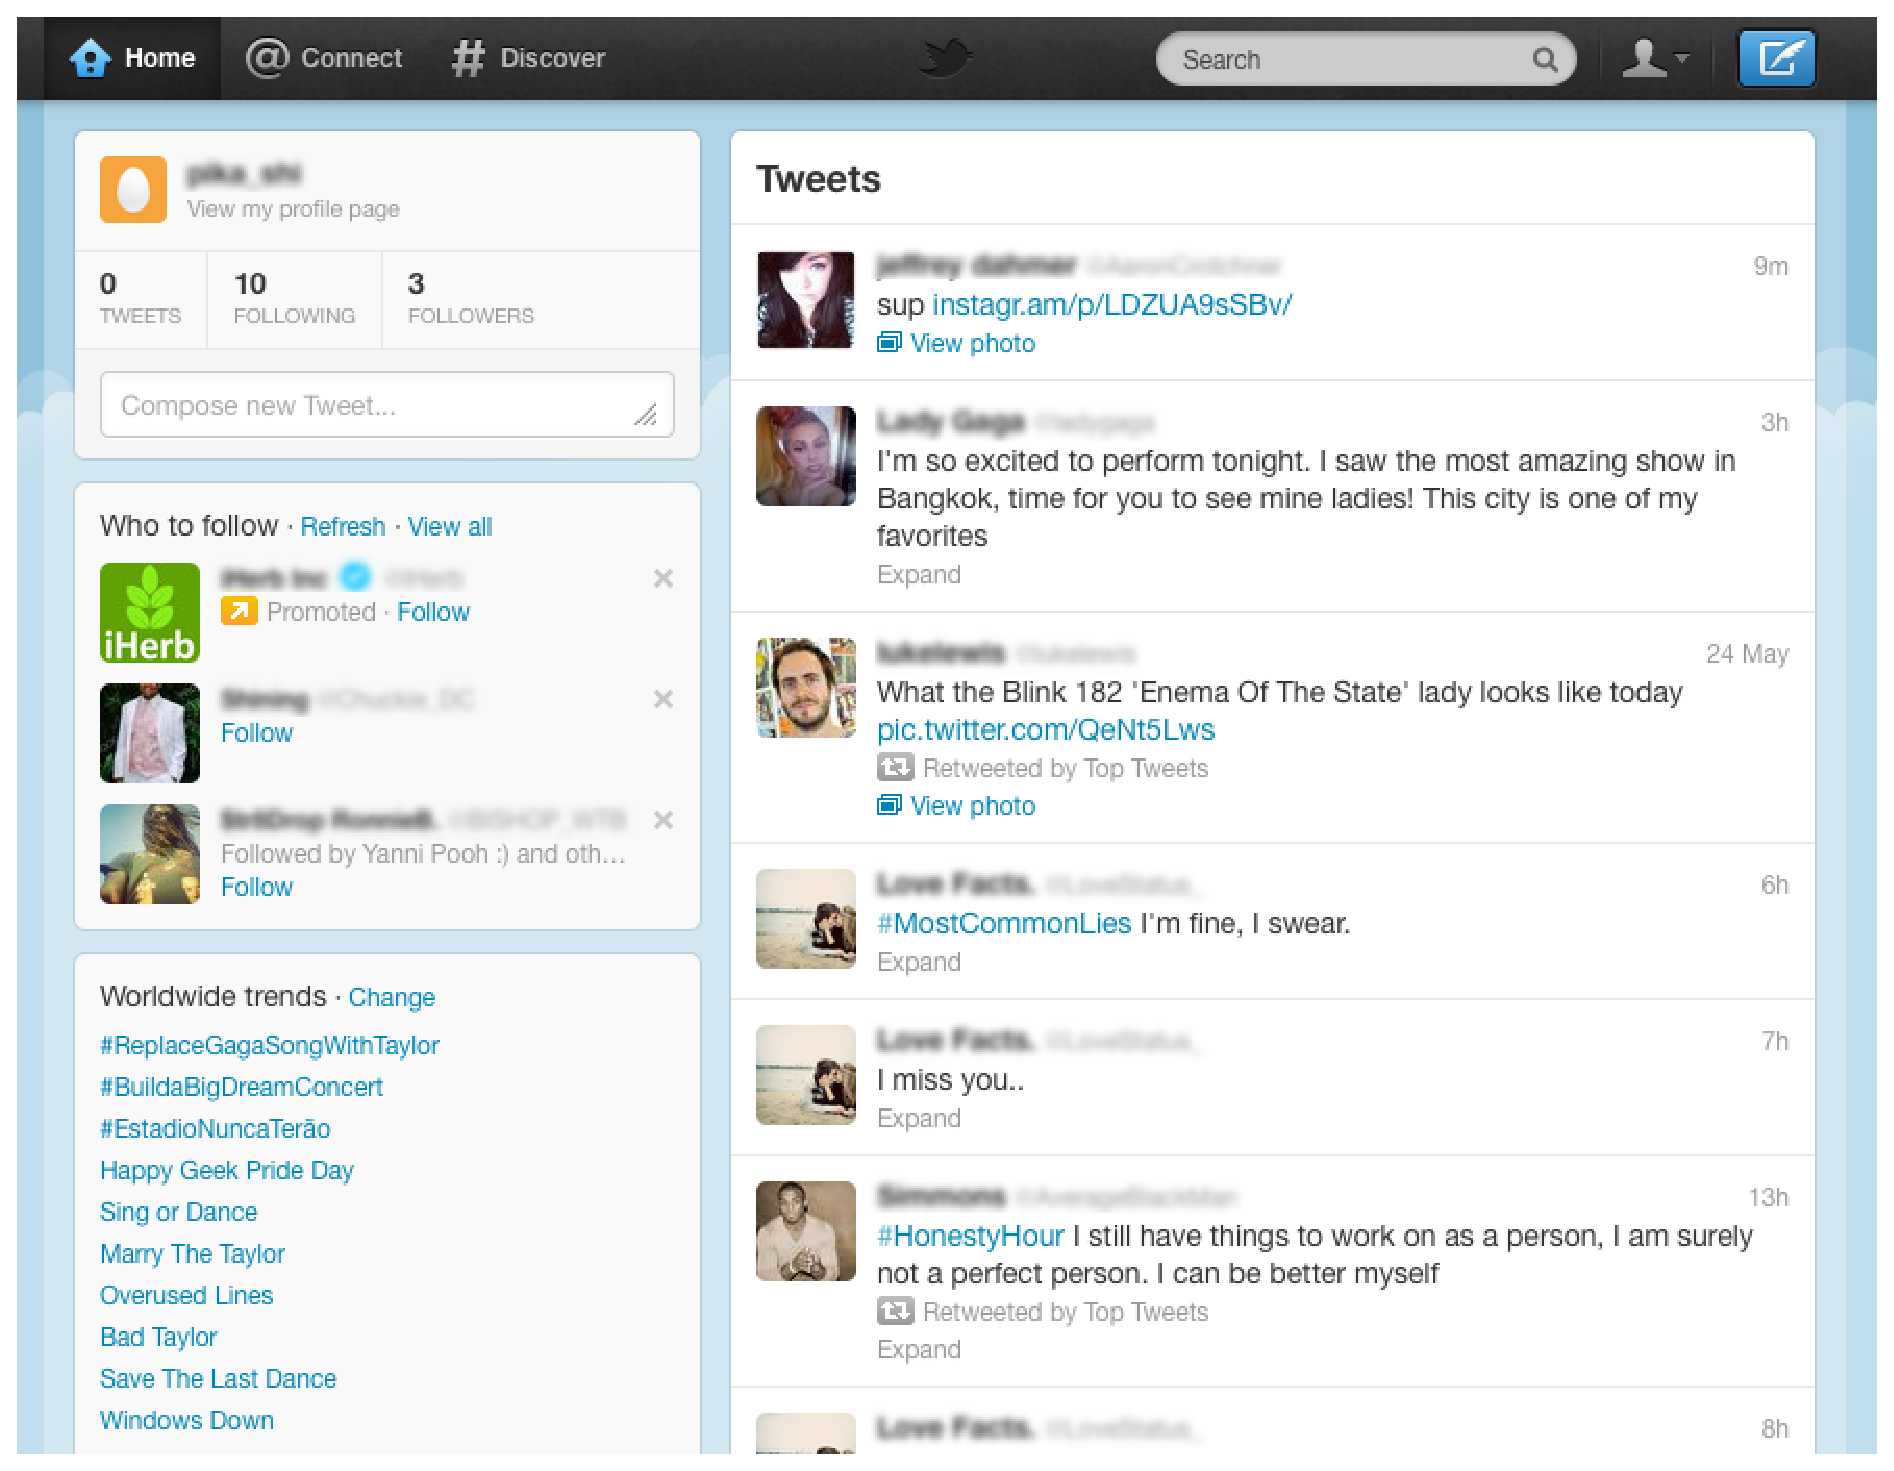
\includegraphics[width=14cm]{images/screen_shot.eps}
 \caption{An example of a user's timeline in Twitter}
\label{fig:twitter}
\end{center}
\end{figure}

As Twitter has characteristics similar to various conventional social
media, so it is used for many purposes.  Some users, e.g., Twitter
accounts owned by major news companies, publish general information on
various topics to the wide public, while some users publish
information specific to certain topics.  There are also users that use
Twitter for the communication with their friends or others.  Because
of this characteristic of Twitter, it has attracted great attention as
a new type of social media.

As explained above, Twitter is used for various purposes.  As a result,
the breadth of target scope of information publishing varies greatly
from users to users.
%tajima:情報発信の対象範囲が様々だというのは説明したとして,次に,その
%場合になぜ対象範囲に基づいてユーザを分類をすることが重要なのか,なぜそ
%ういうことを研究するのに必然性があるのかということについて,ここにもっ
%と書けませんか.
In this study, we propose a method to classify
Twitter users based on how broad the target scope of
their information publishing is, i.e., whether they publish information
to the wide public or publish information to specific groups of users.
In the former case, we say \emph{``target specificity is
low''}, and in the latter case, we say \emph{``target specificity
is high''}.

In our classification method, we use the information on the
consistency among the followers of each user.  If most of the
followers of a user have some noticeable characteristics in common, we
determine that the user publishes information only to users that have
some specific interests or characteristics.  On the other hand, if the
followers of the user have no common noticeable characteristics, it
means that the user is followed by a wide variety of users, and we
determine that the user publishes information to the wide public.

In this study, we also focus on the causes of such target specificity.
We propose a method of determining why target scope of a given user,
which has been classified as a user with high target specifity, is
restricted to some specific type of users.  A large portion of Twitter
users have high target specificity, and the causes of their target
specificity vary from users to users.  For example, some users use
Twitter for the communication with the friends, or for announcing some
information to members of a certain organization.  Messages by such a
user may include various topics and may not be restricted to some
specific topic, but they intend to publish information only to
specific users.  Therefore, their target specificity is high.  On the
other hand, a user who publishes technical information about computer
programming does not have specific users in his mind, but their
messages include only specific topics, i.e., programming, and they
publish information only to users who are interested in programming.
Such a user also have high target specificity.

We roughly classify the causes of target specificity into two types:
(1) topic specificity, i.e., target specificity of a user is high
because the user publishes information on some specific topics, and
(2) user specificity, i.e, target specificity of a user is high
because the user publishes information to a specific group of users.
A ``specific group of users'' means a set of users which can be
defined extensionally, such as friends of some users or members of
some organization.  A set of users which can be defined only
intensionally, e.g., a set of users that are interested in
programming, is not regarded as a ``specific group'' here.

We classify users based on the causes of their high target specificity
by constructing a classifier which determines whether a
user belongs only to category (1), only to category (2), or belong to
both category (1) and (2).  Our classifier uses various features of
users which correlate with each category.  Figure~\ref{fig:Flow} shows
main components of our method and information flow among them.

\begin{figure}[t]
\begin{center}
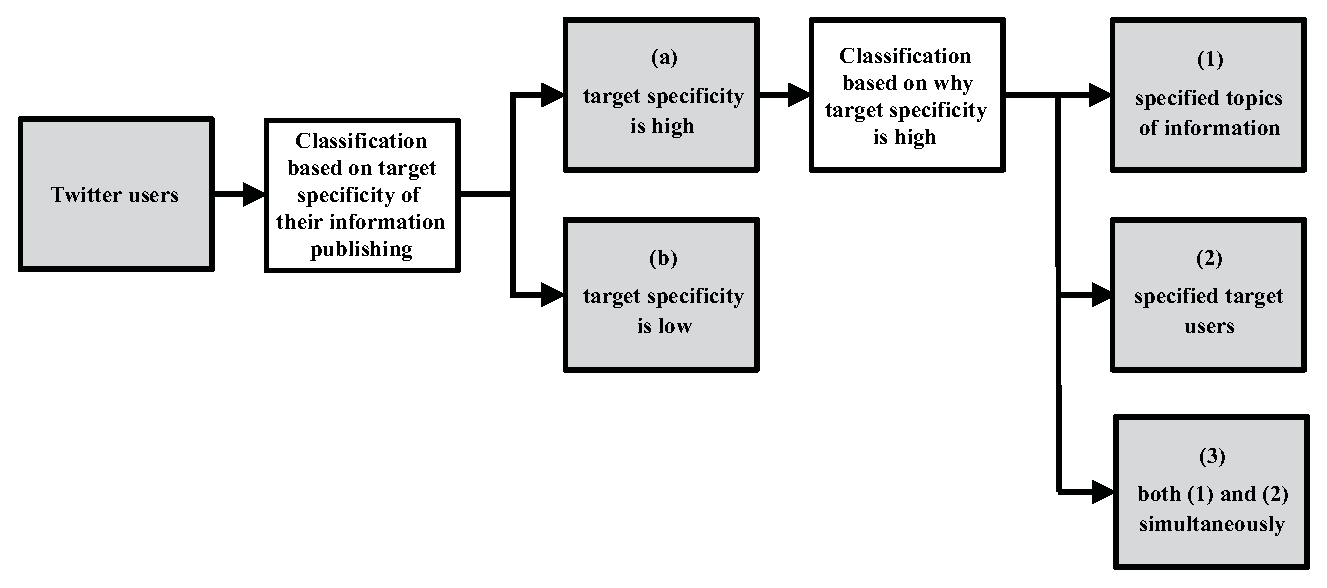
\includegraphics[width=14cm]{images/flow.eps}
 \caption{Main components of our method and information flow among them}
\label{fig:Flow}
\end{center}
\end{figure}

On the Web, it is hard to know what kinds of users each Web page
targets to.  In Twitter, however, we can guess what kinds of users
each user targets to by examining the followers of the user.  By using
this information, we can determine whether a given user has high
target specificity or not.

Twitter user classification by our method can be utilized in Twitter
search systems.  In current Twitter search systems, we input query
keywords and receive messages including the keywords.  In these
systems, however, a search result includes messages with various
target scope.  As a result, it frequently happens that messages
relevant to the querying user are buried in many messages whose target
scope do not include the querying user.  For example, when a user
submits a query ``MacBook Air'' to the Twitter search system, what
kinds of messages he needs depends on the situation.  The user may
need public news about MacBook Air, may need technical information
about MacBook Air, or may need ordinary users' reviews of MacBook Air
in order to decide to or not to buy a MacBook Air.  In the current
Twitter search systems, however, these different types of messages are
mixed in a search result.  In such a case, we can use our Twitter user
classification method in order to classify messages in the search
result, so that messages that the user wants are not buried in many
other types of messages.

The contribution of this paper is summarized as follows.

\begin{itemize}
\item We propose a new classification scheme of Twitter users which is
based on target specificity their information publishing.
\item We show a method of classifying Twitter users in the scheme above.
\item We also show a method of determining the causes of high target
specificity for users that are classified as users with high target specificity.
\end{itemize}

The rest of this paper is organized as follows.  Next chapter explains
some related work and clarify the relationship between our study and
the related work.
We then define target specificity of information publishing and
formulate our problem in \ref{sec:Target Specificity}. In
\ref{sec:Target Specificity}, we also discuss why target scope of some
user is restricted to some specific type of users.  In
\ref{sec:ClassificationMethod1}, we explain the method of classifying
Twitter users based on their target specificity of information
publishing.  In addition, we explain the method of determining the
causes of target specificity of the users classified as high target
specificity users in \ref{sec:ClassificationMethod2}.  Then in \ref{sec:Experiment},
we show the results obtained from experiments we conducted to
evaluate our methods.  \ref{sec:Conclusion} concludes the paper.

\section{Related Work}
\label{sec:Related Work}

With explosive widespread use of microbloggs, studies about
them have recently become frequently performed.  There are various
studies of microblogs, e.g., studies of the
classification microblogging messages from various point of
view\cite{irani2010study}, studies of ranking microblogging messages by
the content relevance and so on\cite{duan2010empirical}, or studies of focusing on
real-time nature of migroblogs\cite{takemura2012tweet,mathioudakis2010twittermonitor}.

In this study, we focus on the fact that Twitter is used for various
purposes. We attempt to classify Twitter users based on the
wideness of target scope of their information publishing, and apply this
classification scheme on Twitter search and so on.  We explain the
following previous studies: studies about the purpose of use of
microbloggs in \ref{subsec:Purpose of Use}, studies of
classifying Twitter users and measuring their influence in
\ref{subsec:Twitter User}, studies useful for finding microblogging
messages related to only certain Twitter users in \ref{subsec:Some
User}, and studies about Twitter search in \ref{subsec:Twitter Search}.
We make the position of this study clear by introducing these studies.

\subsection{Purpose of Use of Microblogs}
\label{subsec:Purpose of Use}

There has been many studies about the purpose of use of microblogs. Java
et al.\cite{java2007we} analyzed the topological and
geographical structure of Twitter's social network and attempted to
understand the user intentions and community structure in microblogging
services.  As a result, they found that the main types of user
intentions are daily chatter, conversation, sharing information and
reporting news.  Kwak et al.\cite{kwak2010twitter} reported that Twitter
is used both as a social network service and as a media for
disseminating or gathering information, and in its follower-following
topology analysis they have found a non-power-law follower distribution,
a short effective diameter, and low reciprocity, which all mark a
deviation from known characteristics of human social networks.  There
are many more studies about the purpose of use of microbloggs\cite{wu2011says,zhao2009and}.

Ehrlich et al.\cite{ehrlich2010microblogging} conducted a
content analysis and examined the use of public microbloggs
(Twitter) for public and private use by comparing internal
microblogs (in the workspace).  As a result, there were
significant differences in content.  The internal microblogs
were generally used to solicit technical assistance or as part of a
conservation.  The public microblogs were used for status
updates and to share general information.

In recent years, Twitter, one of public microblogs, is often
used for not only publishing information to the public but also having a
relationship to only a certain community.  It is able to be said that
this study focuses on the fact that we use Twitter for various purposes.

\subsection{Classification of Twitter Users and Measuring their Influence}
\label{subsec:Twitter User}

There are many studies focusing on Twitter users, e.g., studies of
classification them from various point of view, and studies which measure
their influence.

Studies focusing on the classification of Twitter users are performed
frequently and they have a wide variety of classification schemes, e.g.,
the classification based on their attributes such as political
orientation or ethnicity by leveraging observable information such as
the user behavior, network structure, and linguistic content of their
posting messages\cite{pennacchiotti2011machine}, the classification
into spam users or not by extracting observable features from the
collected candidate spam profiles, e.g., number of friends, text on the
profile, age, and so on\cite{lee2010social}, and the classification
into human users, bots, and cyborgs using entropy measures, machine
learning, and so on\cite{chu2010tweeting}.  Bots refer to automated
programs posting on Twitter, and cyborgs refer to either bot-assisted
humans or human-assisted bots, i.e., interweave characteristics of both
humans and bots.

The classification scheme proposed by Yan et
al.\cite{yan2013classifying} deeply relates to ours.  They proposed
methods to classify Twitter users into open accounts and closed
accounts.  An open account is the
account with a purpose for advertising or spreading information such as
a shop, a singer, a news agency, and so on.  On the other hand, a closed
account is the
account with a purpose for making friends or communication such as a
user who publishes messages about daily log, feeling show, and so on.
This classification scheme is close to ours, but does not coincide with
ours because open accounts don't often publish information to the public
widely.  For example, a user who publishes very technical information
about programming to unspecified users is an open account though he is a
target user.

In microblogs like Twitter or other social network services
like Facebook, users correspond to nodes in social network graphs. As
well as the classification of users, i.e., nodes in the graphs, the
classification of edges, i.e., relationship between a user and his
followers, is related to our study. Leskovec et
al.\cite{leskovec2010predicting,leskovec2010signed} classified edges in
SNS into positive edges such as friendship, and negative edges such as
antagonism. Kunegis et al.\cite{kunegis2009slashdot} also use positive
edges and negative edges in Slashdot, a message board service, in order
to rank the users. Cheng et al.\cite{cheng2011predicting} and Hopcroft
et al.\cite{hopcroft2011will} studied the problem of predicting
reciprocity between two given Twitter users.

There are also studies focusing on measuring influence of Twitter
users.  Jianshu et al.\cite{weng2010twitterrank} focused on the problem of
identifying influential users of microblogs.  Cha et
al.\cite{cha2010measuring} analyzed the influence of them
by employing three measures that capture different perspectives:
indegree, retweets, and mentions.  Then they measured the dynamics of
influence across topic and time.  If target specificity of Twitter users
defined in this study is high, there is a high probability that they
have a big influence on Twitter, but how low target specificity of a
user is does not necessarily coincide with how big his influence is.

\subsection{Find Messages Related to Some Twitter Users}
\label{subsec:Some User}

There are also studies useful for finding of microblogging messages
related to only a part of Twitter users.

Sakaki et al.\cite{sakaki2010earthquake} proposed a method of monitoring
messages in Twitter and detecting occurrences of a specific kind of event
in the real world, such as earthquakes or typhoons.  They produced a
probabilistic spatiotemporal model for the target event that can find
the center and the trajectory of the event location.  Ikawa et
al.\cite{ikawa2012location} attempt to discover the location where a
message was generated by using its textual content.  They learned
associations between a location and relevant keywords from past
messages, and guessed where a new message came from.  It is able to be
said that these studies are useful for finding messages in Twitter
related to certain geographical areas.

Sriram et al.\cite{sriram2010short} proposed approach effectively
classifies the message to a predefined set of generic classes such as
News, Events, Opinions, Deals, and Private Messages.  They proposed to
use a small set of domain-specific features extracted from the user's
profile and text.  Nishida et al.\cite{nishida2011tweet} proposed a
method that uses data compression for classifying an unseen tweet as
being related to an interesting topic or not.  It is able to be
said that these studies are useful for finding messages in Twitter
specified to certain topics.

As mentioned above, there are many studies useful for finding microblogging
messages related to only a part of Twitter users in various points of
view.  But these points of view exist in great number, so it is not an
efficient approach to find these messages from each point of view.
Thus in this study, we attempted to measure Twitter users' target
specificity of information publishing in an integrated way.  In
addition, we roughly classified various causes of target specificity
into two categories.

\subsection{Twitter Search}
\label{subsec:Twitter Search}

The characteristic of search on microblogs is different
from that of Web search\cite{broder2002taxonomy} in that search on
microblogging services can get information in real
time\cite{busch2012earlybird} and not only information published by the
mass media but also much casual information published by
individuals\cite{java2007we}.  Thus, a purpose of use of search on
microblogs often becomes a subject of study.

Teevan et al.\cite{teevan2011twittersearch} observed that people use
Twitter search to find temporally relevant information, e.g., breaking
news, real-time content, and popular trends, and information related to
people, e.g., content directed at the searcher, information about
people of interest, and general sentiment and opinion.  Furthermore,
they compared Twitter search with Web search and found that search
results on Twitter included more social chatter and social events, and
those on the Web included more basic fact and navigation content.
Massoudi et al.\cite{massoudi2011incorporating} proposed a retrieval
model for searching messages on microblogs for a given topic
of interest and a dynamic query expansion model for messages retrieval.
And Nagamoti et al.\cite{nagmoti2010ranking} described several
strategies for ranking messages of microblogging services in a
real-time search engine.

As mentioned above, there are many studies about search on microblogs,
and contents of them are greatly various.  In this study, we
focus on the purpose of use of microblogs, and attempt to
apply it to Twitter Search.  It is able to be said that this study also
focuses on search on microblogs just like studies explained
above, but there has not been studies based on Twitter user's target specificity
of information publishing so far.
\section{Target Specificity of Twitter Users}
\label{sec:Target Specificity}

In this chapter, we discuss the target specificity of Twitter users, the
measure of to what degree target scope of their information publishing
is specified, and define it.  Then we also discuss why target scope of
their information publishing is specified.

\subsection{Definition of Target Specificity}
\label{subsec:Definition}

In this study, we consider target specificity of Twitter users, as
the measure of to what degree target scope of their information publishing is
specified.  More formally, we define \emph{target specificity} of a
Twitter user as to what degree the user set supposed to be included in
target scope of his information publishing is inclining to a
part of all Twitter users, i.e., to what extent this user set deviates
from the user set randomly sampled from all Twitter users.  In this
paper, we express target specificity of the Twitter user $u$ as
$\mathit{TargetSpecificity}(u)$. This formula takes a range of $[0, 1]$.

For example, a user mainly publishing technical information about
programming is supposed to publish information to programmers.  So
users who are interested in this information are inclining toward a part
of Twitter users.  Thus, it is supposed that target specificity of
the user is high.

On the other hand, a user publishing information about world news
publishes information useful for the public widely.  So the public is
supposed to be interested in this information, and the deviation between
users who are interested in this information and users randomly sampled
from all Twitter users may be very small.  Thus, it is supposed
that target specificity of the user is low.

As mentioned above, target specificity of Twitter users is defined
as to what extent the user set supposed to be included in target scope
of his information publishing deviates from the user set randomly
sampled from all Twitter users.  Thus, the fact that target
specificity of a user is high does not necessarily coincide with the
fact that there is high similarity between users supposed to
be included in target scope of his information publishing each
other.  For example, users supposed to be included in target scope of
information publishing of a user publishing information about
earthquake in a certain area are probably consistent in the area they live in,
and so his/her target specificity is supposed to be high.  But their
other characteristics, e.g., age, sex, interests, communities they
belong to, and so on, vary from user to user.  Thus it is not be able to
be said that they have high similarity each other.  In other words, even
if there are various types of users in target scope of his
information publishing, we consider that target specificity of the
user is high as long as the majority of users in the target scope are
consistent in at least one attribute.

In this paper, we determine a threshold $\delta$. If target
specificity of a user is higher than $\delta$, we call him a
\emph{target user}, and if lower, we call him a \emph{non target
user}.  More formally, we define them as follows:

\vspace{-1ex}
\[
  \begin{cases}
   u\mbox{ is a } target\mbox{ }user, & \mbox{if}\
   \mathit{TargetSpecificity}(u) > \delta \\
   u\mbox{ is a }non\mbox{ }target\mbox{ }user, & \mbox{otherwise}.
  \end{cases}
\]
\vspace{-2ex}

\subsection{Why Target Specificity is High}
\label{subsec:The Causes}

In this subchapter, we discuss what causes target specificity of a
user, i.e., why target scope of his information publishing is
specified.  As a result of our analysis, this is roughly classified into
two causes: $(1)$ because he publish information specified for certain
topics, and $(2)$ bacause he publish information to the users
specified extentionally.  We discuss their two causes of the target
specificity in the follow.

\begin{description}
\bf {\item[(1)] Specified topics of information extensionally}
\label{item:Topic}
\end{description}

The first cause of target specificity of a user is because
he publishes information specified to a few topics extensionally,
whether he publishes information to the users specified extentionally or
not.  For example, a user mainly publishing technical
information about programming is supposed to publish information to
unspecified users, but it is considered that target scope of
his information publishing is specified because he specifies the
topic of information, i.e., programming.  Furthermore, a user mainly
publishing information about a certain conference is supposed to publish
information to the users who attend the conference or are interested in
it.  Thus it is considered that target scope of his
information publishing is specified.

The way to specify topics of information is roughly classified into two
cases.  In the first case, a user specifies topics based on demographic
data, e.g., age, settled areas, sex, occupation, career, and so on.  It
is able to be said that a user publishing weather information in a
certain area specifies topics based on demographic data.  In the second
case, a user specifies topics based on psychographic data e.g., taste,
hobby, values, and so on.  It is able to be said that a user
publishing information about cooking specifies topics based on
psychographic data.

\begin{description}
\bf{\item[(2)] Specified target users extensionally}
\label{item:User}
\end{description}

The second cause of target specificity of a user is because
he publishes information specified to some users extensionally
whether he specifies topics of his publishing
information or not.  For example, a user communicating with his friends
publishes various contents of information, but it is considered that
target scope of hisher information publishing is specified because
heshe specifies users extensionally, i.e., he publishes
information to the closed users, i.e., his friends.  Furthermore, a user
mainly getting in touch with members of a certain club publishes
information to the closed users specified extensionally, i.e., the club
members.  Thus it is considered that target scope of
his information publishing is specified.

Sometimes, both $(1)$ and $(2)$ simultaneously cause the target specificity of a
user.  For example, a user who publishing information to
the members of the artist's fan club publishes information specified not
only users of his information publishing, i.e., the members of the
artist's fan club, but also the topic of information, i.e., the latest news
about the artist and so on.  Furthermore, it is also true in case of a
user notifying students in a certain university of the news toward
them because he publishes information specified extensionally, i.e.,
students of the university, and the
topics of information, i.e., the news toward them.  In addition, some users use
Twitter for the both purpose of publishing information of a certain
topic and communicating with their friends.  It is able to be said that
such users are also an example of the case that both $(1)$ and $(2)$ simultaneously
cause the target specificity of a Twitter user.
\section{Classifying Users Based on Target Specificity}
\label{sec:ClassificationMethod1}

In this chapter, we explain the method of classifying Twitter users
based on target specificity of their information publishing defined
in \ref{sec:Target Specificity}.

\subsection{Assumptions and Outline of the Method}
\label{subsec:Assumptions}

In this study, we assume that a follower set of a user is the
user set randomly sampled from users included in target scope of his
information publishing.  Thus, we focus on the follower set of a user we
intend to classify.

A user publishing information to the public widely, e.g., a user
publishing information about world news, is supposed to be followed
by various types of users.  On the other hand, followers of a user
publishing information specified in certain users are supposed to be
consistent in a certain noticeable character.  For example, a user
publishing technical information about programming is supposed to be
mainly followed by programmers, and a user communicating with his
friends is supposed to be mainly followed by his friends.

Based on the above, we classify a user whether his followers are consistent
in a certain noticeable character and difficult to suppose to be
randomly sampled from all Twitter users, or his followers are not
consistent in any noticeable characters.  Figure~\ref{fig:High
Consistency} (a) shows the case of followers of a user being consistent
in the noticeable character $A$.  In such a case, his followers are
supposed to incline toward a part of all Twitter users, thus we consider
that the more consistent his followers are in a certain noticeable
character, the higher his target specificity is.

In addition to this parameter: whether followers of a user are
consistent in a certain noticeable character or not, we consider
whether his follower set are covered with consistency subsets which
cover intermediately widely.  Here, \emph{a consistency subset} denotes
a subset which have consistency in a certain noticeable character.  As
show in Figure~\ref{fig:High Consistency} (b), in regard to followers of
a user, when half of them are consistent in the noticeable character $A$
and the others are consistent in the character noticeable $B$.  It is
not able to
be said that they are consistent in one noticeable character, but
his follower set are covered with two consistency subsets cobering the
set intermediately widely.  In such a case, we consider that his
target specificity is high.

{\footnotesize
\begin{figure}[t]
\begin{center}
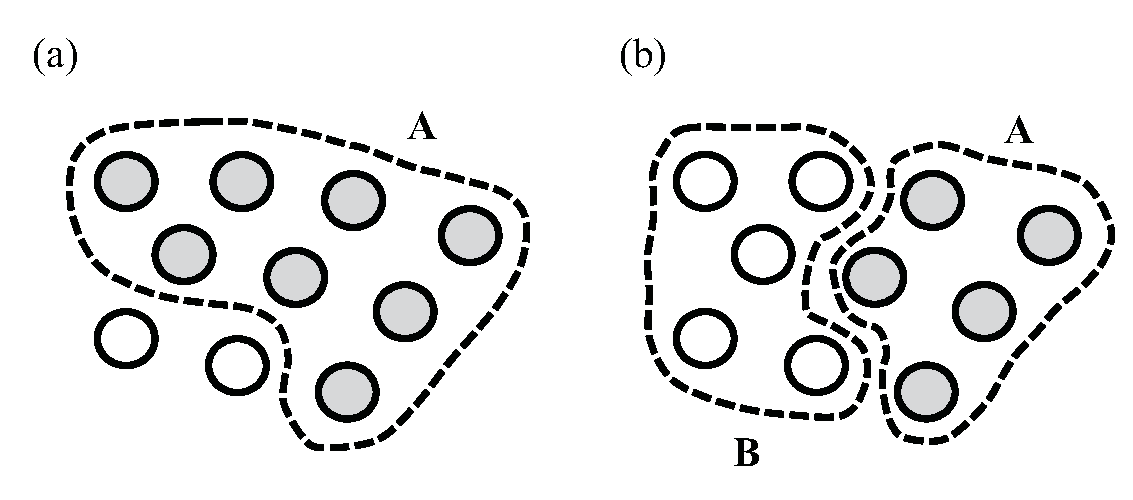
\includegraphics[width=14cm]{images/high_consistency.eps}
 \caption{Two examples of high target specificity}
\label{fig:High Consistency}
\end{center}
\end{figure}
}

These two parameters are summarized as follows:

\begin{description}
\item[(a)] The more consistent followers of a user are in a certain
           noticeable character, the higher his target specificity
           is, and
\item[(b)] The more covered his follower set is with consistency
           subsets covering the set intermediately widely, the higher his
           target specificity is.
\end{description}

Target specificity of a user is quite high when his followers
are consistent in one noticeable character, and it becomes lower as they
do not become consistent in any noticeable characters.

\subsection{Classification Algorithm}
\label{subsec:Algorithm}

In this subchapter, we explain the algorithm of computing a score of
target specificity of a user $u$ based on the outline mentioned in the
above subchapter.

First, we collect all consistency subsets included in $F_u$, the
follower set of $u$.  Then, in regard to each subset $S_{F_uc}$, which
is consistent in
the character $c$ included in $F_u$, we compute
$\mathit{SubsetScore}(S_{F_uc})$ which denotes to what degree users in
$S_{F_uc}$ are consistent in $c$. We will propose two models
computing $\mathit{SubsetScore}(S_{F_uc})$ in \ref{subsec:Scoring}.

Second, in the descending order of $\mathit{SubsetScore}(S_{F_uc})$, we give
this score to each follower $f$ in $S_{F_uc}$ as
$\mathit{UserScore}_{\mathit{att}}(f)$, where $\mathit{att}$ means a
attribute measuring consistency, and we will explain two attributes in
\ref{subsec:Attributes}. Here, we do not give a score to $f$ if
he/she already has a score. Then, we repeat this step over all
$\mathit{SubsetScore}(S_{F_uc})$.  In regard to users who are not given
a score after the above repeat, we set $0$ to them.  In other words, in
regard to each $f$ of $u$, we give
$\mathit{UserScore}_{\mathit{att}}(f)$ to the largest
$\mathit{SubsetScore}(S_{F_uc})$ of $S_{F_uc}$ in which $f$ is included,
as follows:

\vspace{-1ex}
\[
 \mathit{UserScore}_{\mathit{att}}(f) = \max_{S_{F_uc} \in F_u}
 \{\mathit{SubsetScore}(S_{F_uc})|\;f \in S_{F_uc}\}.
\]
\vspace{-2ex}

Then, we take average of all $\mathit{UserScore_{\mathit{att}}(f)}$ for
$\mathit{SpecificityScore_{\mathit{att}}(u)}$, a score of target
specificity of $u$ using the attribute $\mathit{att}$, as follows:

\vspace{-1ex}
\[
 \mathit{SpecificityScore}_{\mathit{att}}(u) = \frac{1}{|F_u|}
 \sum_{f \in F_u} \mathit{UserScore}_{\mathit{att}}(f).
\]
\vspace{-2ex}

For example, suppose the case shown in Figure~\ref{fig:Algorithm}.
We assume that a follower set of a user $u$ have three consistency
subsets: $A$, $B$, and $C$, and $\mathit{SubsetScore}(A)$,
$\mathit{SubsetScore}(B)$, and $\mathit{SubsetScore}(C)$ are $3$, $2$,
and $1$ respectively.  In the descending order of
$\mathit{SubsetScore}(S_{F_uc})$, i.e., in order of $A$, $B$, and $C$,
we give scores to each follower $f$ as
$\mathit{UserScore}_{\mathit{att}}(f)$ as shown in
Figure~\ref{fig:Algorithm}.  Finally, we compute average of
$\mathit{UserScore}_{\mathit{att}}(f)$ and take $2.6$ for
$\mathit{SpecificityScore_{\mathit{att}}(u)}$.

{\footnotesize
\begin{figure}[t]
\begin{center}
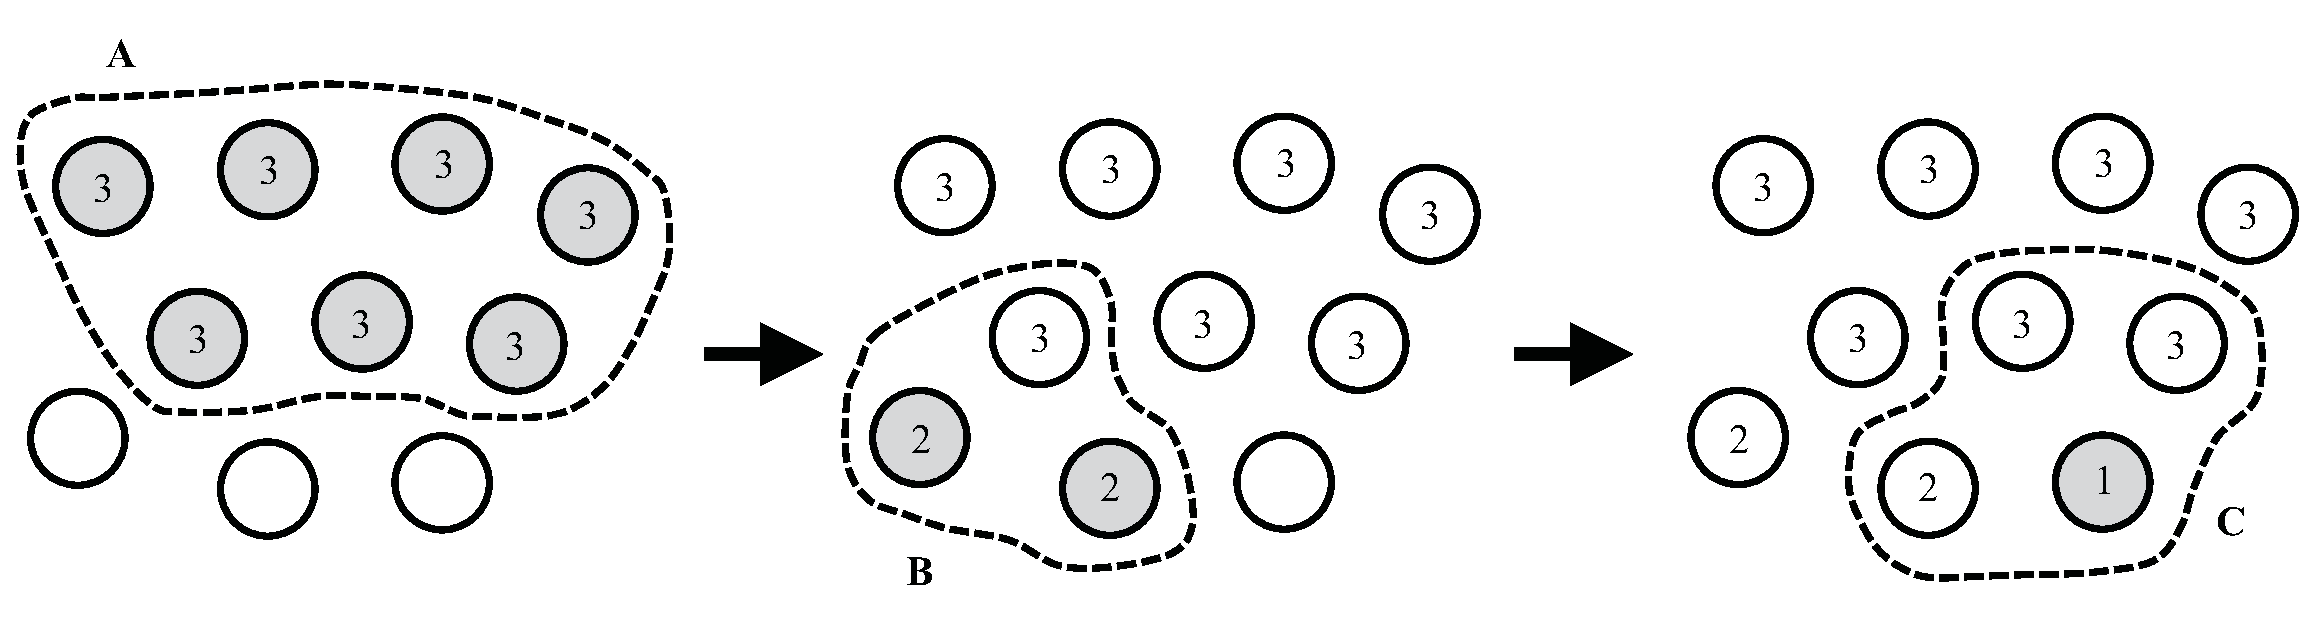
\includegraphics[width=14cm]{images/algorithm.eps}
 \caption{A case of the algorithm flow}
\label{fig:Algorithm}
\end{center}
\end{figure}
}

This is how we compute a score of target specificity of $u$ using the
attribute $\mathit{att}$.  Below is a summary of the algorithm:

\begin{description}
\item[1.]  we collect all consistency subsets included in the follower set,
\item[2.]  we score each consistency subset based on to what extent users
           in it are consistent in a certain noticeable character,
\item[3.]  in the descending order of the above scores, we repeatedly
           give the score to each user in the subset, and
\item[4.]  we take average of scores for a score of target specificity.
\end{description}

\subsection{Scoring Models of Consistency Subsets}
\label{subsec:Scoring}

In this subchapter, we explain a couple of models in the follow: the
probabilistic model and the subtracting model which compute
$\mathit{SubsetScore(S_{F_uc})}$ mentioned in \ref{subsec:Algorithm}

\subsubsection{Probablistic Model}
\label{subsubsec:Probablistic}

In this model, in regard to the consistency subset $S_{F_uc}$ being
consistent in the character $c$ in the follower set $F_u$, we consider
that how low the probability that the user set of the same size as $F_u$
randomly sampled from all Twitter users includes the subset
being consistent in $c$ and whose size is $|S_{F_uc}|$ and over.
The lowness of the probability means that $S_{F_u}$ is inclining to
a part of all Twitter users, so it is able to be said that
$S_{F_uc}$ has consistency in a noticeable character if the probability
is low.  Thus, the lower the probability is, the higher score we give.
On the other hand, if the probability is
not so low,  the deviation between $S_{F_uc}$ and the user set randomly
sampled from all Twitter users may be small, and it is difficult to say
that $S_{F_uc}$ has consistency in a noticeable character.  Thus, we
give a low score in this case.

In addition to this parameter: how low the probability mentioned above
is, we consider the covering rate of $S_{F_uc}$ to $F_u$.  The higher
the covering rate of $S_{F_uc}$ to $F_u$ is, the higher score we give.
Based on these two parameters, we compute $\mathit{SubsetScore(S_{F_uc})}$.

These two parameters are summarized as follows.
\begin{itemize}
\item The lower the probability that the user set of the same size as $F_u$
randomly sampled from all Twitter users includes the subset
being consistent in the same character as the character of $S_{F_uc}$
and whose size is $|S_{F_uc}|$ and over, the higher score we give.
\item The higher the covering rate of $S_{F_uc}$ to $F_u$ is, the higher
      score we give.
\end{itemize}

Then, we define this model more formally.  First, we compute
$P(S_{F_uc})$, the probability that the user set of the size of $|F_u|$
randomly sampled from the set of all Twitter users includes the subset
being consistent in $c$ and whose size is $|S_{F_uc}|$ and over, by the
formula below:

\vspace{-1ex}
\[
 P(S_{F_uc}) = \int_{|S_{F_uc}|}^{n} \binom{n}{x} p^x (1-p)^{n - x}
 dx,\;\;\;\;\;n = |F_u|,\;\;\;\;\;p = \frac{|S_{Ac}|}{|A|}
\]
\vspace{-2ex}

\noindent{where $A$ is the set of all Twitter users, and $S_{Ac}$ is the
subset which is consistent $c$ in the character included in $A$.  The
parameter $x$ in the above formula is based on a binomial distribution.}

In addition, by adding the covering rate of $S_{F_uc}$ to $F_u$ to the
above parameter, we compute $\mathit{SubsetScore(S_{F_uc})}$.  However,
there is some possibility that $P(S_{F_uc})$ is excessively low because
$S_{F_uc}$ has a remarkable character, e.g., the character only a few
users of all users have, in spite of the size of $S_{F_uc}$ is very
small.  In this model, we expect that the consistency subset covers the
follower set at least intermediately widely.  So in such a case, we do
not give any scores to $S_{F_uc}$.  More formally, we determine a
threshold $\gamma$ which cuts down the above case.

Then, we compute $\mathit{SubsetScore(S_{F_uc})}$ by the formula below:

\vspace{-1ex}
\[
  \displaystyle \mathit{SubsetScore}(S_{F_uc}) = \begin{cases}
    \displaystyle \frac{|S_{F_uc}|}{|F_u|} \log (1 - P(S_{F_uc})) &
    \mbox{if } \displaystyle \frac{|S_{F_uc}|}{|F_u|} > \gamma, \\
    \displaystyle \;\;\;\;\;0 & \mbox{otherwise.}
  \end{cases}
\]
\vspace{-2ex}

This is how we compute $\mathit{SubsetScore(S_{F_uc})}$ by using
the probabilistic technique.

\subsubsection{Subtracting Model}
\label{subsubsec:Subtracting}

In this model, in regard to the consistency subset $S_{F_uc}$, we
consider a covering rate of $S_{F_uc}$ to $F_u$ in comparison to a
covering rate of the subset which is consistent in the character $c$ to the set of
all Twitter users.  We call the former \emph{a local rate} and the
latter \emph{a global rate}.  The fact that a local rate is high and a
global rate is low means $S_{F_uc}$ has consistency in a noticeable
character and is including toward a part of all Twitter
users.  If a local rate is low or a global rate is high, it is difficult
to say that $S_{F_uc}$ has consistency in a noticeable character.  Based
on the above, we compute $\mathit{SubsetScore(S_{F_uc})}$ by the formula
below:

\vspace{-1ex}
\[
 \mathit{SubsetScore}(S_{F_uc}) = \max \{\frac{|S_{F_uc}|}{|F_u|} -
 \frac{|S_Ac|}{|A|}, 0\}.
\]
\vspace{-2ex}

In summary, we give a high score in the case of having the two features
simultaneously as follows:

\begin{itemize}
\item a covering rate of $S_{F_uc}$ to $F_u$ is high, and
\item a covering rate of the subset being consistent in the same
      character as the character of $S_{F_uc}$ to the set of all Twitter
      users is low.
\end{itemize}

This is how we compute $\mathit{SubsetScore(S_{F_uc})}$by using
the subtracting technique.

\subsection{Attributes for Extracting Consistency Subsets}
\label{subsec:Attributes}

In this subchapter, we explain a couple of attributes measuring
consistency: common terms in profiles and location information, and
common followees.  By using these attributes, we extract consistency
subsets from the follower set of a user.  We explain these two
attributes in the follow.

\subsubsection{Common Terms in Profiles and Location Information}
\label{subsec:Terms}

As the first attribute measuring consistency, we consider common terms
included in profiles and local information of followers.

There is a high possibility that users belonging to the same community
or having the same interest have the same term in their profiles or
location information in common.  Thus, we extract such terms for
measuring consistency.  Here, we extract only noun phrases, which
characterize their profiles or location information strongly.

Based on the above, we define the method of extracting consistency
subsets more formally.  We compute the consistency subset $S_{F_ut}$
which is consistent in the term $t$ in $F_u$ by the formula below:

\vspace{-1ex}
\[
 S_{F_ut} =  \sum_{f \in F_u} \{f|\;t \in \mathit{Demography}(f) \}
\]
\vspace{-2ex}

\noindent{where $\mathit{Demography}(f)$ is the profile and location information
of $f$.  This is how we extract consistency subsets by using common
terms in profiles and location information.}

\subsubsection{Common Followees}
\label{subsec:Followees}

As the second attribute measuring consistency, we consider common
followees of followers.

Users being consistent in a certain noticeable character often have
the common tendency of the follow.  Users belonging to the same
community are dense on the social graph, so there is a high possibility
that they follow common users in the community.  In addition, followers of
a user publishing technical information about programming is supposed
to follow another user publishing useful information about programming
in common.  Thus, we focus on the tendency of the follow and extract
such followees for measuring consistency.

Based on the above, we define the method of extracting consistency
subsets more formally.  We compute the consistency subset $S_{F_ue}$
which is consistent in the followee $e$ in $F_u$ by the formula below:

\vspace{-1ex}
\[
 S_{F_ue} =  \sum_{f \in F_u} \{f|\;e \in E_f \}
\]
\vspace{-2ex}

\noindent{where $E_f$ is the followee set of $f$.  This is how we extract
consistency subsets by using common followees.}

\subsection{Final Classification Based on Target Specificity}
\label{subsubsec:Final Classification}

In this subchapter, we explain the method of computing target
specificity of a user by using scores computed up to this
point.  In addition, based on target specificity, we also explain the
method of classifying users.

The $\mathit{SpecificityScore}_{{\mathit{att}}}(u)$ computed in
\ref{subsec:Algorithm} is higher in the cases that

\begin{itemize}
\item the more consistent followers of a user are in a noticeable
      character, or
\item the more covered his follower set are with consistency
      subsets covering it intermediately widely.
\end{itemize}

Then, we compute a score of target specificity of $u$. We first
compute $\mathit{SpecificityScore}_{{\mathit{term}}}(u)$, which is using
common terms in profiles and location information as an attribute
measuring consistency mentioned in \ref{subsec:Terms}, and
$\mathit{SpecificityScore}_{{\mathit{followee}}}(u)$, which is using
common followees mentioned in \ref{subsec:Followees}.  Next, we propose
a couple of approaches computing target specificity of $u$ by using the
above two scores in the follow.

\begin{description}
\bf{\item[(1)] Average and maximum of two scores}
\label{item:Avg and Max}
\end{description}

In the first approach, we take the average and the maximum scores of two
scores.  For comparison of two scores, we first normalize them by
computing the deviation values.

Then, we take the average score of two scores for target specificity of
$u$ by the formula below:

\vspace{-4ex}
\[
 \mathit{TargetSpecificity}(u) = {\rm avg} \{
 \mathit{SpecificityScore}_{{\mathit{term}}}(u),
 \mathit{SpecificityScore}_{{\mathit{followee}}}(u)\}
\]
\vspace{-4ex}

In addition to the average score, we also take the larger one of two
scores for target specificity of $u$, because the larger one is supposed to
characterize target specificity more strongly than the other.  More
formally, we compute $\mathit{TargetSpecificity}(u)$ by the formula
below:

\vspace{-4ex}
\[
 \mathit{TargetSpecificity}(u) = \max \{
 \mathit{SpecificityScore}_{{\mathit{term}}}(u),
 \mathit{SpecificityScore}_{{\mathit{followee}}}(u)\}
\]
\vspace{-4ex}

This is how we compute a score of target specificity of $u$ using the
approach taking the average and the maximum of two scores.

\begin{description}
\bf{\item[(2)] Binary classifier with the features of two scores}
\label{item:Binary Classifier}
\end{description}

In the second approach, we construct a binary classifier with the feature of
two scores.  If target specificity of $u$ is high, we set
$\mathit{TargetSpecificity}(u)$ to 1, and otherwise we set it to 0.  We
adopt SVM and decision tree as a classifier.

%This is how we compute a score of target specificity of $u$ using the
%approach using a binary classifier with the feature of two scores.

Then we classify users based on target specificity.  We determine a
threshold $\delta$ which can classify target users and non target users
accurately the most, and we classify them by $\delta$.  More formally,
we classify them as follows:

\vspace{-1ex}
\[
\begin{cases}
u\mbox{ is a } \mathit{target}\mbox{ }\mathit{user}, & \mbox{if}\
\mathit{TargetSpecificity}(u) > \delta \\
u\mbox{ is a }\mathit{non}\mbox{ }\mathit{target}\mbox{ }\mathit{user}, & \mbox{otherwise}.
\end{cases}
\]
\vspace{-2ex}

This is how we classify users into target users and non target users
based on target specificity.
\section{Classifying Users of High Target Specificity}
\label{sec:ClassificationMethod2}

In this chapter, in regards to Twitter users classified into ``the
target specificity is high'' by the method mentioned in the above
chapter, we explain the method of determining why their target
specificities are high based on the result of our analysis mentioned in
\ref{subsec:The Causes}.

\subsection{Architecture of the Classifiers}
\label{subsec:Architecture}

Here, we focus on the two causes of the high target specificity
mentioned in \ref{subsec:The Causes} as follows:
\begin{description}
 \item[(1)] because they publish information specified for certain
            topics, and
 \item[(2)] because they publish information to the users specified
            extensionally,
\end{description}

\noindent{and we determine whether a user we intend to classify
correlates with each cause mentioned above.}

We first determine various features of the user which potentially
correlate with each cause.  Then, based on these features, we construct
the classification method which classifies users into three categories:
(1) their target specificity is high because they publish information
specified for certain topics, (2) because they publish information to
the users specified extensionally, and (3) in the cause of both (1) and
(2).  By classifying users with the above classifiers, we determine why
their target specificities are high.

We adopted SVM and decision tree as a classifier.  Next, we propose a
couple of approaches to classify users into three categories.

\subsubsection{3-class Classifier}
\label{subsubsec:3-class}

In the first approach, we construct a single 3-class classifier using
one-against-one method.  Each result class corresponds to each category:
(1), (2), and (3).  Figure~\ref{fig:classifier} (a) shows architecture
of a 3-class classifier.

\subsubsection{2 Binary Classifiers}
\label{subsubsec:2-binary}

In the second approach, we construct two binary classifiers, each of
which determines (i) whether users publish information specified for
certain topics, amd (ii) whether users publish information to the users
specified extensionally, respectively.  When the results of two
classifiers are \emph{yes} and \emph{no} respectively, we classify them
into the category (1): their target specificity is high because they
publish information specified for certain topics.  When \emph{no} and
\emph{yes}, we classify them into the category (2): because they publish
information to the users specified extensionally, and when \emph{yes}
and \emph{yes}, we classify them into the category (3): in the cause of
both (1) and (2).  Figure~\ref{fig:classifier} (b) shows architecture of
2 binary classifiers.

{\footnotesize
\begin{figure}[t]
\begin{center}
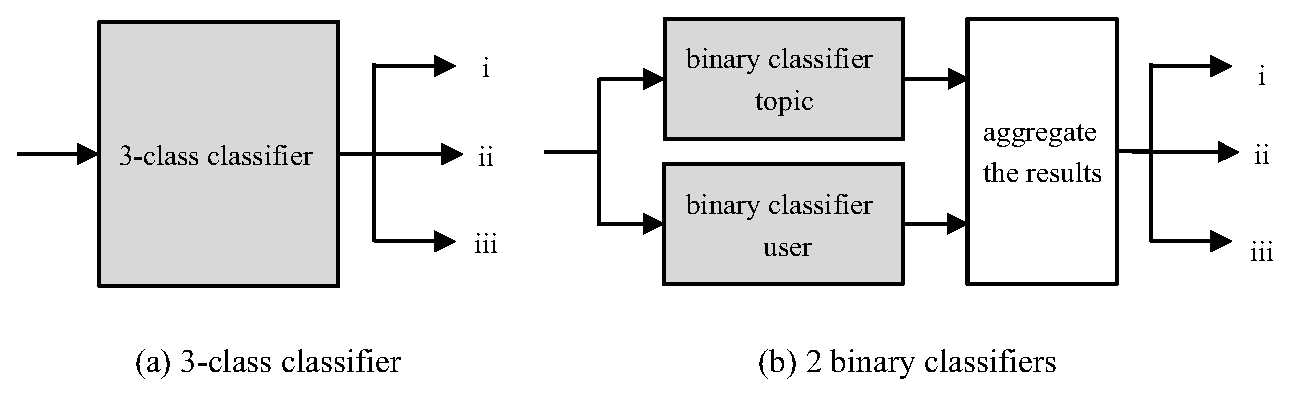
\includegraphics[width=14cm]{images/classifier.eps}
 \caption{Architecture of a couple of classifiers: (a) 3-class
 classifier and (b) 2 binary classifiers}
\label{fig:classifier}
\end{center}
\end{figure}
}

\subsection{Features Used for the Classification}
\label{subsec:Features}

In this subchapter, we explain what features of users we used for the
classification.  All the feature values shown below were normalized to
values between $0$ and $1$.

\begin{description}
\bf {\item[(i)] numbers of followees and followers, and their ratio}
\end{description}

If the user publishes information to unspecified users, there is high
probability that a number of his/her followers is quite large or a
number of his/her followees is quite small.  So in such a case, a ratio
of a number of his/her followees to a number of his/her followers is
supposed to be very small.  Furthermore, if the user publishes
information to the closed users, i.e., his/her friends, his/her club
members, and so on, there is high probability that numbers of his/her
followers and followees are very close because the user is supposed to
have a reciprocal connection with them.  Thus, numbers of followees and
followers, and their ratio are expected to be useful for determining why
their target specificities are high.

We take a logarithm of numbers of followers and followees because the
difference of large numbers of followers and followees are not as
important as the difference of small numbers of followers and followees.

\begin{description}
\bf {\item[(ii)] mutual follow ratio}
\end{description}

There is high probability that the user publishing information to the
closed users has a large mutual follow ratio, i.e., a number of users
with whom one follows one another is large, because the user is supposed
to have a reciprocal connection with them.  Therefore, a mutual follow
ratio is expected to be useful for determining why their target
specificities are high.

\begin{description}
\bf {\item[(iii)] frequency of replies by ``@''}
\end{description}

There is high probability that the user publishing information to the
closed users has a high frequency of replies by ``@'', i.e., the user
replies to his/her followers frequently. In regard to a mutual follow
ratio mentioned in (ii), there are some users publishing information to
unspecified users in spite of a large mutual follow ratio, but in regard
to a frequency of replies by ``@'', there is high probability that the
user publish information to the closed users.  This is because a high
frequency of replies by ``@'' demonstrates that the user is supposed to
have a reciprocal connection with them.  Therefore, a frequency of
replies by ``@'' is expected to be useful for determining why their
target specificities are high.

\begin{description}
\bf {\item[(iv)] partialness of topics in messages}
\end{description}

In regard to a user publishing information specified for certain topics,
topics in his/her messages are often partial.  Thus, we use the
partialness of topics in his/her messages as a feature for the
classification.

Then, we explain how to compute a partialness of topics in messages of
$u$.  We first collect up to 200 messages in order of newness.  Second,
we extract noun phrases from them and we use their phrases as a corpus.
We extract only noun phrases bacause they characterize contents of the
messages strongly.  Then, we determine the topic of each message by
using Latent Dirichlet Allocation (LDA), which is a generative
probabilistic model for collections of discrete data such as text
corpora, by using the above corpus.  Finally, we compute partialness of
topics in messages $\mathit{partialness}(u)$ as follows:

\vspace{-3ex}
\[
 \mathit{partialness}(u) = - \sum_{t \in T_u} p_t \log p_t,\;\;\;\;\;
 p_t = \frac{|\{m|\;m \in M_u,\;\mathit{topic}(m) = t\}|}{|M_u|}
\]
\vspace{-3ex}

\noindent{where $M_u$ is a message set of $u$, $T_u$ is the topic set we
use for computing this feature, and $\mathit{topic}(m)$ is the topic of
a message $m$.  The partialness of topics $partialness(u)$ is the
entropy of $M_u$ on the topic.  This is how we compute a partialness of
topics in messages.}
\section{Experiments and Discussions}
\label{sec:Experiment}

In this chapter, we conduct experiments to evaluate our methods proposed
in \ref{sec:ClassificationMethod1} and \ref{sec:ClassificationMethod2},
and present the results obtained from them.  In addition, we discuss our
methods based on the results.

\subsection{Data Set}
\label{subsec:Data Set}

We collected the data set from the real Twitter data by using Twitter
API.

We first randomly selected 1,000 Twitter users whose timezone is Japan.
At this time, we omitted users who are followed from nobody and who post
no tweet in order to select only active users.  Then, we divided them in
two sets equally, i.e., each of which include 500 users.

Second, we had 6 experienced Twitter users as participants, all of whom
are male graduate students in engineering, from 23 to 25 years old.  We
assigned each set to 3 participants, and we asked each participant to
determine one of the following categories each user in the assigned set
is supposed to be in:

\begin{description}
\item[(i)] the user publishes information to the public widely,
\item[(ii)] the user publishes information specified for certain topics,
\item[(iii)] the user publishes information to the users specified
           extensionally, and
\item[(iv)] the user publishes information (ii) specified for certain
           topics (iii) to the users specified extensionally.
\end{description}

\noindent{These categories correspond to the category (b), (1), (2), (3)
in Figure~\ref{fig:Flow} respectively.}

Then, we selected users whose category at least 2 out of 3 participants
coincide with, and as a result, we were able to collect 93, 320, 375,
and 30 users in the category (i), (ii), (iii), and (iv).  We randomly
selected 90 users from the category (i), and 30 users from (ii), (iii),
and (iv) respectively.  We collected these 180 users in total, and we
used them as the data set.  Table~\ref{breakdown} shows the breakdown of
the data set: average and standard deviation of numbers of followers,
 followees, and tweets in each category.

\newcolumntype{I}{!{\vrule width 1.5pt}}
\newcommand{\bhline}[1]{\noalign{\hrule height #1}}
\begin{table}[t]
\caption{Average and standard deviation of numbers of followers,
 followees, and tweets in each category \label{breakdown}}
\begin{center}
\begin{tabular}{c|cIc|c|c|c}
\multicolumn{2}{cI}{} & \makebox[4em]{i} & \makebox[4em]{ii} &
 \makebox[4em]{iii} & \makebox[4em]{iv} \\ \bhline{1.5pt}
 \multirow{2}{*}{follower} & average & 475,679 & 58,142 & 573 & 82,942  \\
 & standard deviation & 535,894 & 171,784 & 1,389 & 262,161 \\ \hline
 \multirow{2}{*}{followee} & average & 11,274 & 3,353& 598 & 1,568 \\
 & standard deviation & 37,906 & 7,218 & 1,545 & 3,594 \\ \hline
 \multirow{2}{*}{tweet} & average & 9,763 & 9,992 & 8,829 & 5,677 \\
 & standard deviation & 14,607 & 23,572 & 29,505 & 6,600 \\
\end{tabular}
\end{center}
\end{table}

\begin{table}[t]
\caption{Average and standard deviation of numbers of followers,
 followees, and tweets in each category \label{ClassifierResultslog}}
\begin{center}
\begin{tabular}{cIc|cccc}
Removed Feature & \makebox[4em]{with all} & \makebox[3em]{i} &
 \makebox[3em]{ii} & \makebox[3em]{iii} & \makebox[3em]{iv} \\
 \bhline{1.5pt}
 3-class SVM & 67.8 & 64.4 & {\bf 72.2} & 67.8 & 65.5  \\ \hline
 2 binary SVMs & 68.9 & 65.6 & 71.1 & 67.8 & 67.8  \\ \hline
 3-class decision tree & 55.6 & 54.4 & 46.7 & 47.8 & 50.0 \\ \hline
 2 binary decision trees & 53.3 & 52.2 & 44.4 & 47.8 & 47.8  \\
\end{tabular}
\end{center}
\end{table}

\begin{table}[t]
\caption{Average and standard deviation of numbers of followers,
 followees, and tweets in each category \label{ClassificationDetailslog}}
\begin{center}
\begin{tabular}{c|cIc|cccc}
\multicolumn{2}{cI}{Removed Feature} & \makebox[4em]{with all} &
 \makebox[3em]{i} & \makebox[3em]{ii} &  \makebox[3em]{iii} &
 \makebox[3em]{iv} \\ \bhline{1.5pt}
 \multirow{2}{*}{SVM} & \makebox[4em]{topic} & 85.6 & 81.1 & {\bf 86.7}
                 & 84.4 & 84.4  \\
 & user & 83.3 & 84.4 & 84.4 & 83.3 & 82.2 \\ \hline
 \multirow{2}{*}{decision tree} & topic & 72.2 & 68.9 & 65.6 & 72.2 & 74.4 \\
 & user & 75.6 & 76.7 & 74.4 & 71.1 & 70.0 \\
\end{tabular}
\end{center}
\end{table}

Then, for each user, we collected at most 1,000 followers of the user,
and in regard to the followers who follow at most 1,000 users, we also
collected their followees.  We used them in order to evaluate our
methods.

\subsection{Experimental Settings and Libraries}
\label{subsec:Settings}

First, we conducted the experiments evaluating the method of classifying
Twitter users based on the target specificity of their information
publishing mentioned in \ref{}.  We used 90 users classified into the category (i) as target
users, and 90 users classified into the category (ii), (iii), and (iv)
as non target users.  We first computed
$\mathit{SpecificityScore}_{{\mathit{term}}}(u)$ and
$\mathit{SpecificityScore}_{{\mathit{followee}}}(u)$ for each user $u$,
and computed $\mathit{TargetSpecificity}(u)$ based on the above scores.
Then, we determined a threshold $\delta$ which can classifies target
users and non target users accurately the most, and evaluated the
classification results with $\delta$.  When computing
$\mathit{TargetSpecificity}(u)$, we used two models: the probabilistic
model and the subtracting model mentioned in \ref{subsubsec:Scoring},
and compared them.

Second, we conducted the experiments evaluating the method of determing
why the target specificity of the user is high in regard to the target
user.  We extracted users from the category (ii), (iii), and (iv) by 30
users, and used 90 users in total.  We first extracted features
mentioned in \ref{subsec:Classification Step2} from the user.  Then,
based on these features, we constructed 3-class classifiers which
classify users into three categories: (ii), (iii), and (iv), and
evaluated the classification results using 10-fold cross validation.  We
used two learning algorithms: SVM and the decision tree as classifiers,
and compared them.  For SVM, we used
LIBSVM\footnote{\url{http://www.csie.ntu.edu.tw/~cjlin/libsvm/}}, which
is a popular SVM library, with the Gaussian kernel.  For the decision
tree, we used scikit-learn
\footnote{\url{http://scikit-learn.org/stable/modules/tree.html}}.

We used twpro search API\footnote{\url{http://twpro.jp/doc/api/search}}
in order to get a number of users who have a certain term in their
profiles.  We also used
MeCab\footnote{\url{http://mecab.sourceforge.net/}} for morphological
analysis of Japanese sentences in profiles, local information, and
tweets of $u$.  Furthermore, we used
gensim\footnote{\url{http://radimrehurek.com/gensim/}} for using Latent
Dirichlet Allocation (LDA).

実験結果を図\ref{demography},図\ref{follow},図\ref{pr}に示す.
図\ref{demography}は,プロフィール・位置情報を用いて対象限定性を表した手法,図
\ref{follow}は,フォローの傾向を用いて対象限定性を表した手法を表しており,
それぞれスコアの高いものからソートしている.図\ref{pr}は,上記の二つの手
法で求めたスコアをそれぞれ降順にソートし,ターゲット型ユーザを正解
とした場合の,適合率・再現率曲線を表している.また,適合率・再現率曲線の
ベースラインとして,20件のユーザそれぞれのフォロワー数を昇
順にソートし,同じくターゲット型ユーザを正解としたものを用いている.

フォロワー内でのプロフィール・位置情報を用いた手法に関しては,図
\ref{demography}に示すように,ターゲット型ユーザの方が,非ターゲット
型ユーザよりも,対象限定性を表すスコアが高くなっており,これらを明確に分
類することができているといえる.また,図\ref{pr}に示すように,適合
率・再現率曲線も,ベースラインを上回っている.これらの結果より,プロフィー
ル・位置情報を用いて対象限定性を表す手法は,ターゲット型ユーザと非ターゲッ
ト型ユーザを分類するのに有効であるといえる.

フォロワー内でのフォローの傾向を用いた手法に関しても,図\ref{follow}に示
すように,ターゲット型ユーザの方が非ターゲット型ユーザよりも,対象限定性
を表すスコアが平均的に高くなった.しかし,これら二つの間の差は大きくなく,
適合率・再現率曲線に関しては,図\ref{pr}に示すように,ベースライン
を下回る結果となった.これらの原因としては,以下のようなものが考えられる.
\vspace{1ex}


{\bf(1)} 本実験では,フォロワーのフォローの傾向を用いた手法の中で,Twitter
       の日本人ユーザ全体でのフォローの頻度$\mathit{uf}$を求めているが,
       実際には,Twitterに登録しているものの,ほとんど利用していないユー
       ザも多く存在する.そのようなユーザの影響で,$\mathit{uf}$が必要以
       上に小さくなってしまっており,最終的なスコアに十分反映されていな
       いと考えられる.今後は,Twitterユーザ全体ではなく,Twitterのアクティブユーザ
       のみの中からフォローの頻度を求めることで,本問題の改善を図る予定
       である.\vspace{1ex}

{\bf(2)} フォロワー内に強く一貫した傾向がなくても,フォローに共通の傾
       向が見られる場合があると考えられる.本実験において,社会のニュー
       スを発信するユーザのフォロワーの多くが,社会のニュースを発信する
       別のユーザを同時にフォローしているというケースが見られたが,実際
       には,フォロワー内に社会のニュースに興味があるという弱い一貫性は
       あるものの,強く一貫した傾向は見られなかった.\vspace{1ex}

\subsection{実験結果の詳細と分析}
\label{sec:detail}

本節では,実験結果から,正解データとして用いたユーザの分析を行った結果を
示す.表\ref{detail}に,正解データ内のターゲット型ユーザ・非ターゲット型
ユーザのうち,各2ユーザの詳細を表している.各ユーザそれぞれに関して,
\ref{sec:Determine Specificity}節で定義した$\mathit{tf}$が高い3語と,
$\mathit{ff}$が高い3ユーザを示し,実験結果におけるそれらのスコアを示して
いる.

ターゲット型ユーザである@minnanomachi(写真に関するプロジェクトのア
カウント)に関しては,「写真」や「カメラ」といった語のスコアや,カメラ関連
のアカウントのスコアが高くなっており,そのアカウントを特徴付けるような結
果が得られているといえる.同様にターゲット型ユーザである@USJ\_BGM(USJに
関するアカウント)に関しても,「USJ」といった語のスコアや,USJ関連のアカ
ウントのスコアが高くなっている.また,「好き」といった一般に出現頻度の高
い語や,@masason(孫正義)といった広く一般に知られているユーザは,
$\mathit{tf}$や$\mathit{ff}$が高くなっているが,$\mathit{df}$や
$\mathit{uf}$によりそれらのスコアは下がっており,最終的なスコアは非常に小
さくなっていることが分かる.

非ターゲット型ユーザに関しては,「大好き」や「フォロー」といった,一般に
出現頻度の高い語や,@pamyurin(きゃりーぱみゅぱみゅ)や@TDR\_PR(東京
ディズニーリゾートに関するアカウント)といった,広く一般に知られているユー
ザが抽出されているが,$\mathit{df}$や$\mathit{uf}$によりこれらのスコアは
下がっている.特に,プロフィール・位置情報を用いた手法のスコアは全て0となって
いる.

このように,これらの例に関しては,フォロワー集合の中で特徴のある語やフォ
ローの傾向を抽出することができており,提案手法が有効であるといえる.ただ
し,現在の手法では,「写真」と「カメラ」というような同じトピックに関する
語を,完全に独立なものとして扱っている.このような語を関連付けて考え,対
象限定性を求める有効性を向上させることが今後の課題である.

\subsection{アプリケーションの実装}
\label{sec:Application}

本節では,本研究の提案手法を応用した,実装予定のアプリケーションについて
述べる.

本アプリケーションは,提案手法に基づき,Twitterの検索結果を3つのタブに分
類することで,ユーザのTwitter検索を支援するものである.以下に,表示する3
つのタブついてそれぞれ示している.\vspace{1ex}

{\bf (1)} 対象範囲が広いユーザの記事を表示する.ある内容に関する一般的な
ニュースのように,広く一般のユーザが興味を示すような記事を得ることができ
る.\vspace{1ex}

{\bf (2)} あるトピックに特化された情報を発信するユーザの記事を表示する.ある
イベントなどに関する具体的な情報や,あるトピックに関する専門的な情報を得るこ
とができる.\vspace{1ex}

{\bf (3)} クローズドなユーザ集合に情報を発信するユーザの記事を表示する.
ある内容に関する一般ユーザの反応などといった,個人のつぶやきなどを得る
ことができる.\vspace{1ex}

このように分類することで,自分の求めている情報を効率よく取得することがで
きると考えている.また,\ref{sec:Elements}節で,あるトピックに特化されており,
かつクローズドなユーザ集合に情報を発信するユーザが存在する旨を述べたが,
そのような記事は,上記の(2)と(3)の両方のタブに表示する予定である.
\section{Conclusion}
\label{sec:Conclusion}

In this study, we focused on the fact that the wideness of target scope of
information publishing in Twitter varies greatly among users, and
proposed the method to classify Twitter
users from the point of view of how widely target scope of their
information publishing is, i.e., whether they publish information to the
public widely or publish information specified in certain users.

First, we defined target specificity of a user, as the
measure of to what degree target scope of his information publishing is
specified.  Second, based on this definition, we proposed the algorithm
computing a score of target specificity.  In this algorithm, we
focused on two parameters: (a) whether followers of a user are
consistent in a certain noticeable character or not, and (b) whether the
follower set of a user is covered with consistency subsets covering it
intermediately widely or not.
For computing the score, we proposed a couple of models computing
scores of consistency subsets: the
probabilistic model and the subtracting model, and a couple of
attributes for extracting consistency subsets from the follower set of a
user: common terms in profiles and location information and common
followees.
Then, we finally proposed four types of methods of classifying users
into target users and non target user based on the score.  We conducted
experiments to compare the performance of the methods, and the results
suggested that the method using a binary SVM classified users with the
highest accuracy.  The results also suggested that common terms in profiles
and location information were more useful for extracting consistency
subsets than common followees.

In addition, in this study, in regard to users classified into
``target specificity is high'' by the above method, we proposed the
the method of determining why their target
specificity is high.  We first analysed the causes of high target
specificity, and we classified users into three
categories based on them: (1) their target specificity is high because
they publish information specified for certain topics,
(2) because they publish information to the users specified extensionally, and
(3) in the cause of both (1) and (2).  Then, we constructed
a couple of approaches to classify them into three categories: a 3-class
classifier and 2 binary classifiers, based on various features of the
user which potentially correlate with each cause.  Our experimental
results suggested that a 2 binary SVM classified users with the highest
accuracy. The results also suggested that the two causes (1) and (2)
were highly independent of each other.

We believe that our proposed methods are applicable to some applications
e.g., Twitter search systems, and they will enrich users' experience on
Twitter.

\acknowledgments
I would like to express my sincere gratitude to my supervisor,
Professor Keishi Tajima for his valuable advises and helpful
discussions.  I deeply appreciate Proffessor Yasushi Sakurai and
Associate Professor Yasuhito Asano for spending precious time for
valuable discussions.  I would also like to thank the other lab members
for their supports for our research.

\nocite{*}
\bibliographystyle{kuissort}
\bibliography{thesis}

\end{document}